% BDE Guide --- Chapter 3: Planning Your BDEs Across Four Years
\chapter{Planning Your BDEs Across Four Years}
\label{ch:planning}

\begin{quote}
\emph{``A degree is a schedule, not just a checklist.''} Where you place BDEs matters as much as which BDEs you pick. A good plan keeps semesters balanced, reserves AU for late surprises, and never forces you into a 24~AU overload to graduate.
\end{quote}

\noindent\fbox{\parbox{\dimexpr\linewidth-2\fboxsep-2\fboxrule}{%
\textbf{From zero: we define Degree Audit, STARS, overload, and S/U before using them.} No prior NTU registration experience assumed.}}
\vspace{0.4em}

\section*{Learning Outcomes}
After this chapter you will be able to:
\begin{enumerate}[label=(L\arabic*)]
    \item interpret a four-year study plan and place BDEs sensibly across semesters;
    \item read Degree Audit correctly (Satisfied / In-Progress / Outstanding);
    \item state overload rules, normal semester load, and when overloading is (not) advisable;
    \item plan around internship (SC3920) and FYP/MPE-heavy final year;
    \item handle STARS bidding, waitlists, and late BDE swaps without panic.
\end{enumerate}

% ============================================================
\section{A Sample Four-Year BDE Distribution}
\label{sec:four-year-plan}

The programme core is front-loaded: Y1--Y2 carry 15--18~AU of compulsory SC/MH modules per semester. Y3 S2 is dominated by the 10~AU Professional Internship (SC3920). Y4 is MPE + FYP (or 3 extra MPE). BDEs fill the gaps.

\begin{table}[h]
\centering
\small
\renewcommand{\arraystretch}{1.22}
\begin{tabular}{@{}l l p{5.8cm} r@{}}
\toprule
Year / Sem & Core load (approx.) & BDE slot & BDE AU \\
\midrule
Y1 S1 & 15--16~AU (SC1003/04/05, MH1812, ICC) & 1 BDE if timetable allows (e.g., HP1000) & 0--3 \\
Y1 S2 & 16--18~AU (SC1006/07/08, SC2000/02) & 0--1 BDE (light if core is heavy) & 0--3 \\
Y2 S1 & 15~AU (SC2001/05/06, SC2203/08) & 1 BDE (business or lang.~1) & 3 \\
Y2 S2 & 12--15~AU (SC2207 + MPE start) & 1 BDE (lang.~2 or HSS) & 3 \\
Y3 S1 & 14--16~AU (SC3099 4~AU + MPEs) & 1 BDE (entrepreneurship / arts) & 3 \\
Y3 S2 & \textbf{10~AU internship} + 1 ICC/MPE & 0 BDE (internship is full-time) & 0 \\
Y4 S1 & MPE/FYP 8--12~AU & 1--2 BDEs (clear remaining) & 3--6 \\
Y4 S2 & MPE/FYP 8--12~AU & 1 BDE (final buffer) & 3 \\
\midrule
\multicolumn{3}{r}{\textbf{Total BDE}} & \textbf{18--21} $\to$ \textbf{20} target \\
\bottomrule
\end{tabular}
\caption{Sample BDE distribution (single-degree, no second major, FYP path). Adjust per your actual core load and internship timing. The 20~AU target is curriculum-page counting; PDF F-Core bucketing shows 21~AU for the same courses.}
\label{tab:bde-timeline}
\end{table}

\begin{remark}[Why not front-load all BDEs?]
Three reasons: (i)~prerequisites --- some desirable BDEs (e.g., BM2501 Business Analytics) expect Y2 standing; (ii)~timetable --- Y1 cores have fixed lecture slots that clash with popular BDEs; (iii)~GPA smoothing --- spreading BDEs lets you balance exam-heavy and project-heavy semesters (see Table~\ref{tab:bde-workload} in Ch.~\ref{ch:popular-bde}).
\end{remark}

\begin{figure}[h]
\centering
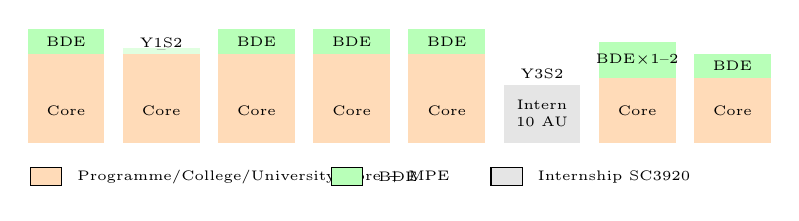
\begin{tikzpicture}[scale=0.78,every node/.style={font=\scriptsize}]
% Timeline bars: 8 semesters
\foreach \i/\label in {0/Y1S1,1/Y1S2,2/Y2S1,3/Y2S2,4/Y3S1,5/Y3S2,6/Y4S1,7/Y4S2} {
  \pgfmathsetmacro{\x}{\i*1.55}
  % Core bar (orange)
  \pgfmathsetmacro{\coreh}{1.45}
  \ifnum\i=5 \def\coreh{0.95}\fi % internship sem shorter core bar
  \ifnum\i>5 \def\coreh{1.05}\fi % Y4 lighter
  \fill[orange!28] (\x,0) rectangle (\x+1.25,\coreh);
  \node[font=\tiny,align=center] at (\x+0.625,\coreh+0.18) {\label};
  \node[font=\tiny] at (\x+0.625,0.52) {Core};
}
% BDE bars (green) on top, varying height
\fill[green!28] (0,1.45) rectangle (1.25,1.85); \node[font=\tiny] at (0.625,1.65) {BDE};
\fill[green!12] (1.55,1.45) rectangle (2.80,1.55); \node[font=\tiny,color=gray] at (2.175,1.50) {--};
\fill[green!28] (3.10,1.45) rectangle (4.35,1.85); \node[font=\tiny] at (3.725,1.65) {BDE};
\fill[green!28] (4.65,1.45) rectangle (5.90,1.85); \node[font=\tiny] at (5.275,1.65) {BDE};
\fill[green!28] (6.20,1.45) rectangle (7.45,1.85); \node[font=\tiny] at (6.825,1.65) {BDE};
\fill[gray!20] (7.75,0) rectangle (9.00,0.95); \node[font=\tiny,align=center] at (8.375,0.48) {Intern\\10 AU};
\fill[green!28] (9.30,1.05) rectangle (10.55,1.65); \node[font=\tiny] at (9.925,1.35) {BDE$\times$1--2};
\fill[green!28] (10.85,1.05) rectangle (12.10,1.45); \node[font=\tiny] at (11.475,1.25) {BDE};
% Legend
\node[fill=orange!28,draw,minimum width=0.4cm,minimum height=0.22cm] at (0.3,-0.55) {};
\node[font=\tiny,anchor=west] at (0.65,-0.55) {Programme/College/University Core + MPE};
\node[fill=green!28,draw,minimum width=0.4cm,minimum height=0.22cm] at (5.2,-0.55) {};
\node[font=\tiny,anchor=west] at (5.55,-0.55) {BDE};
\node[fill=gray!20,draw,minimum width=0.4cm,minimum height=0.22cm] at (7.8,-0.55) {};
\node[font=\tiny,anchor=west] at (8.15,-0.55) {Internship SC3920};
\end{tikzpicture}
\caption{Schematic BDE placement across eight semesters (Y3 S2 internship has no BDE). Heights are schematic; actual AU per semester is in Table~\ref{tab:bde-timeline}. Leave at least one BDE buffer for Y4 in case of timetable clashes or failed bids.}
\label{fig:bde-timeline}
\end{figure}

\paragraph{Buffer rule.} Plan to finish BDEs by Y4 S1, leaving Y4 S2 as buffer. Students who postpone 6+~AU of BDE to the very last semester risk a timetable clash forcing an overload or delayed graduation.

% ============================================================
\section{Degree Audit: The Single Source of Truth}
\label{sec:degree-audit}

\begin{definition}[Degree Audit]
Degree Audit is the official, personalised checklist in StudentLink (Academic $\to$ Degree Audit) that maps every course you have taken, are taking, and plan to take into the correct AU bucket (University Core, College Core, Programme Core, MPE, BDE). It shows Satisfied (green), In-Progress (yellow), and Outstanding (red) for each requirement. If Degree Audit says a requirement is unsatisfied, it \emph{is} unsatisfied --- regardless of what any PDF or senior says.
\end{definition}

\begin{figure}[h]
\centering
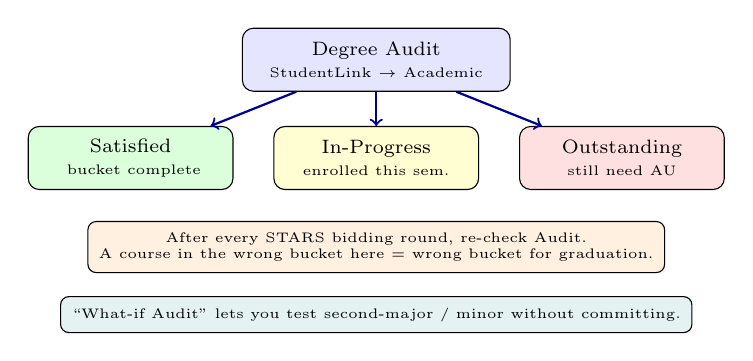
\begin{tikzpicture}[scale=0.78,every node/.style={font=\scriptsize}]
\node[draw,rounded corners=4pt,fill=blue!10,minimum width=3.4cm,minimum height=0.8cm,align=center] (audit) at (0,2.0) {Degree Audit\\{\tiny StudentLink $\to$ Academic}};
\node[draw,rounded corners=4pt,fill=green!14,minimum width=2.6cm,minimum height=0.8cm,align=center] (sat) at (-4.0,0.4) {Satisfied\\{\tiny \textcolor{green!50!black}{\bfseries \checkmark} bucket complete}};
\node[draw,rounded corners=4pt,fill=yellow!18,minimum width=2.6cm,minimum height=0.8cm,align=center] (prog) at (0,0.4) {In-Progress\\{\tiny enrolled this sem.}};
\node[draw,rounded corners=4pt,fill=red!12,minimum width=2.6cm,minimum height=0.8cm,align=center] (out) at (4.0,0.4) {Outstanding\\{\tiny still need AU}};
\draw[->,thick,blue!55!black] (audit) -- (sat);
\draw[->,thick,blue!55!black] (audit) -- (prog);
\draw[->,thick,blue!55!black] (audit) -- (out);
\node[draw,rounded corners=3pt,fill=orange!12,inner sep=4pt,align=center,font=\tiny] at (0,-1.05) {After every STARS bidding round, re-check Audit.\\A course in the wrong bucket here $=$ wrong bucket for graduation.};
\node[draw,rounded corners=3pt,fill=teal!10,inner sep=4pt,align=center,font=\tiny] at (0,-2.15) {``What-if Audit'' lets you test second-major / minor without committing.};
\end{tikzpicture}
\end{figure}

\paragraph{How to use it for BDEs.}
\begin{enumerate}
    \item After STARS enrolment each semester, open Degree Audit and confirm the new course landed in the BDE bucket (not ``Unallocated'' or MPE).
    \item If a BDE appears under ``Unallocated'' (e.g., an SC-coded extra that the system thinks is MPE), email your programme coordinator to reallocate --- do not leave it until Y4.
    \item Use ``What-if Audit'' to simulate adding a second major or minor and see how many BDE AU it consumes.
\end{enumerate}

% ============================================================
\section{Semester Load, Overload, and S/U}
\label{sec:overload}

\begin{definition}[Semester load \& overload]
NTU defines a \emph{normal load} of roughly 16--20~AU per semester (5--6 courses). The \emph{maximum load without special approval} is typically 20--21~AU; beyond that is \emph{overload} and requires academic approval (good GPA, advisor sign-off). The absolute cap per semester is usually 24~AU. Internship semester (SC3920, 10~AU) is an exception --- you take fewer or no additional courses alongside it.
\end{definition}

\begin{definition}[S/U option]
Satisfactory/Unsatisfactory (S/U) lets you take a course without it affecting GPA (S $=$ pass, U $=$ fail, neither enters GPA). At NTU, S/U eligibility is restricted --- typically only BDEs and some ICC courses qualify, and only up to a fixed AU cap (check Academic Regulations for your cohort). Programme Core and MPE generally \emph{cannot} be S/U'd.
\end{definition}

\begin{table}[h]
\centering
\small
\renewcommand{\arraystretch}{1.22}
\begin{tabular}{@{}p{4.0cm} p{7.5cm}@{}}
\toprule
Rule of thumb & Why \\
\midrule
Keep 17--20~AU/semester & Sustainable; leaves time for CCAs, projects, interviews. \\
Avoid 22+ AU unless GPA $\ge 4.0$ & Overload approval is not guaranteed; burnout risk is real. \\
Do not S/U a BDE you need for signal & Employers/grad schools see S, not the grade; S hides a good grade too. \\
Reserve 3--6~AU BDE for Y4 & Buffer for timetable clashes or a failed/dropped BDE. \\
Check STARS vacancy before planning & Popular BDEs (HP1000, AB1601) fill in minutes; have backups. \\
\bottomrule
\end{tabular}
\caption{Overload and planning heuristics for CS students.}
\label{tab:overload-heuristics}
\end{table}

\paragraph{STARS bidding tips.}
\begin{itemize}
    \item STARS (Student Automated Registration System) allocates courses by vacancy and priority (programme cores first, then MPE, then BDE). BDEs are lowest priority --- vacancies are tightest.
    \item Have 2--3 backup BDEs per slot. If your first choice is full, bid the backup immediately; do not wait for add/drop hoping a slot opens.
    \item Add/drop week (first week of semester) is your last chance to swap without penalty --- attend both the enrolled and desired BDE's first class if you are waitlisted.
\end{itemize}

% ============================================================
\section{Second Major, Minor, and BDE Trade-offs}
\label{sec:second-major-trade}

A second major (e.g., Business, Mathematics) or minor consumes AU that would otherwise be BDE. The ``What-if Audit'' shows the exact trade:

\begin{center}
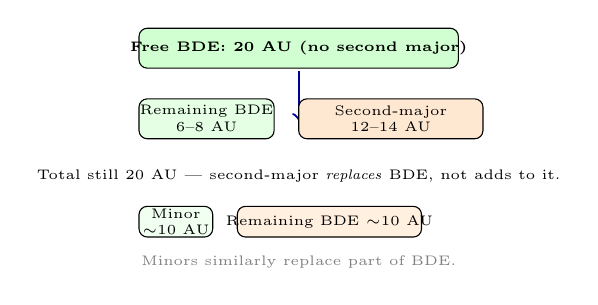
\begin{tikzpicture}[scale=0.78,every node/.style={font=\scriptsize}]
\draw[fill=green!18,rounded corners=3pt] (0,0) rectangle (5.2,0.65);
\node[font=\tiny\bfseries] at (2.6,0.32) {Free BDE: 20 AU (no second major)};
\draw[->,thick,blue!60!black] (2.6,-0.05) -- (2.6,-0.85);
\draw[fill=green!10,rounded corners=3pt] (0,-1.15) rectangle (2.2, -0.50);
\node[font=\tiny,align=center] at (1.1,-0.82) {Remaining BDE\\6--8 AU};
\draw[fill=orange!18,rounded corners=3pt] (2.6,-1.15) rectangle (5.6,-0.50);
\node[font=\tiny,align=center] at (4.1,-0.82) {Second-major\\12--14 AU};
\node[font=\tiny,align=center] at (2.6,-1.75) {Total still 20 AU --- second-major \emph{replaces} BDE, not adds to it.};
\draw[fill=green!6,rounded corners=3pt] (0,-2.25) rectangle (1.2,-2.75);
\node[font=\tiny,align=center] at (0.6,-2.50) {Minor\\$\sim$10 AU};
\draw[fill=orange!12,rounded corners=3pt] (1.6,-2.25) rectangle (4.6,-2.75);
\node[font=\tiny,align=center] at (3.1,-2.50) {Remaining BDE $\sim$10 AU};
\node[font=\tiny,gray] at (2.6,-3.15) {Minors similarly replace part of BDE.};
\end{tikzpicture}
\end{center}

If you declare a second major, your ``free BDE'' shrinks --- but the second-major courses themselves broaden you, so the spirit of BDE is preserved. Decide by Y2 S1; late switches waste AU.

% ============================================================
\section{Chapter Notes}
Load and overload rules per NTU Academic Regulations and CCDS programme structure (AY2024--25). STARS procedures per NTU StudentLink documentation. S/U rules vary by cohort and programme --- confirm in Degree Audit and Academic Regulations.

% ============================================================
\section{Exercises}
\label{sec:ch03-exercises}
\begin{enumerate}[label=E3.\arabic*, leftmargin=*, itemsep=0.8em]
    \item \textbf{Semester balance.} You must take SC2006 (group-heavy, 20~h/wk with project) and SC2005 (exam-heavy) next semester. You also need 3~AU of BDE. Which BDE workload profile (exam-heavy vs.\ group-heavy) balances better, and why?
    \item \textbf{Audit triage.} After STARS, Degree Audit shows your new BDE under ``Unallocated'' instead of BDE. What happened, and what do you do?
    \item \textbf{Buffer planning.} A friend plans to finish all 20~AU of BDE by Y3 S1 and leave Y4 with only MPE/FYP. Is this risky or safe? Give two failure modes if it goes wrong.
    \item \textbf{Second-major math.} A second major requires 30~AU. How many ``free'' BDE AU remain under the 20~AU bucket if you declare it? What Degree Audit feature lets you test this before committing?
\end{enumerate}
% End of Chapter 3
